\documentclass[12pt]{article}
\usepackage[pdftex]{graphicx}
\usepackage{listings}
\usepackage{verbatim}

\pagestyle{empty}
\setcounter{secnumdepth}{2}
\newcommand{\systemName}{Task Manager }
\topmargin=0cm
\oddsidemargin=0cm
\textheight=22.0cm
\textwidth=16cm
\parindent=0cm
\parskip=0.15cm
\topskip=0truecm
\raggedbottom
\abovedisplayskip=3mm
\belowdisplayskip=3mm
\abovedisplayshortskip=0mm
\belowdisplayshortskip=2mm
\normalbaselineskip=12pt
\normalbaselines

\begin{document}

\vspace*{0.5in}
\centerline{\bf\Large Design Document}

\vspace*{0.5in}
\centerline{\bf\Large Team 1}

\vspace*{0.5in}
\centerline{\bf\Large 11 March 2012}

\vspace*{1.5in}
\begin{table}[htbp]
\caption{Team}
\begin{center}
\begin{tabular}{|r | c|}
\hline
{\bf Name} & {\bf ID Number} \\
Jonathan Bergeron & 9764453 \\
Marc-Andr\'{e} Faucher & 9614729 \\
Jeffrey How & 9430954 \\
Dmitry Kuznetsov & 5679311 \\
William Ling & 9193480 \\
Thomas Paulin & 9333630 \\
Alain Sakha & 9770836 \\
Kai Wang & 5652723 \\
\hline
\end{tabular}
\end{center}
\end{table}

\clearpage

\section{Introduction}

The purpose of this document is to provide the reader with an understanding of the design of the \systemName system. Each section provides differing levels of detail. We begin with a high-level description of the architectural design followed by a detailed description of the Model, View and Controller subsystems. We conclude the document with examples of execution scenarios to provide the reader with concrete examples of design data flow.

\section{Architectural Design} \label{sec:arch}

A foundational background of the overall system is required in order to understand the goals of the respective subsystems and their relationships.

\subsection{Architectural Diagram}

\begin{figure}[htbp]
\begin{center} 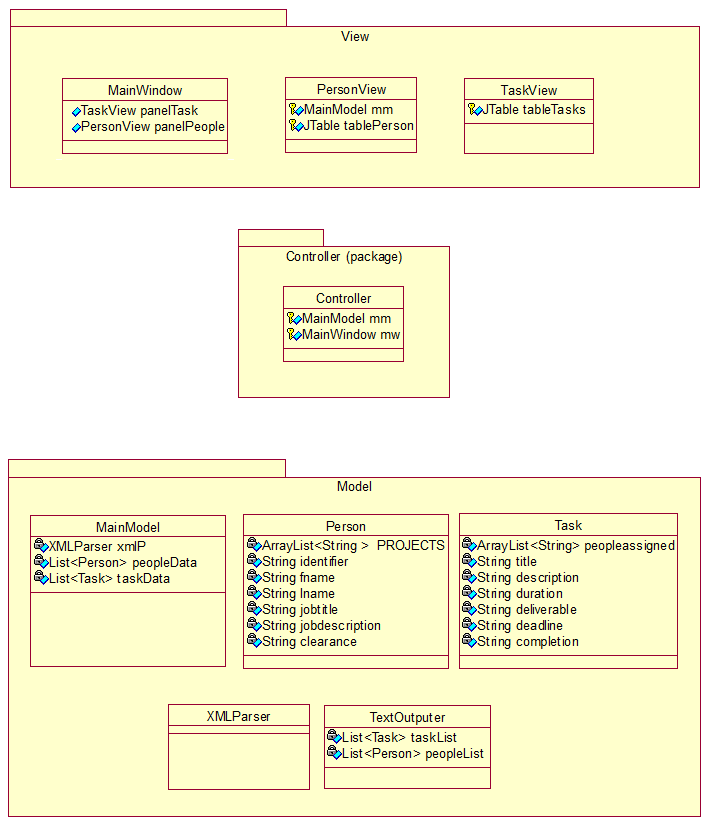
\includegraphics[scale=.5]{Diagrams/archDiagram.png} \end{center}
\caption{Architectural Design Diagram}
\label{fig:arch-diagram1}
\end{figure}

The \systemName consists of three main subsystems; Model, View, and Controller. This design was chosen due to its feasibility and synergy with simple Graphical User Interfaces. 

The Model is the hub for all essential data and data manipulation. It interfaces with input/output classes to read and write data to XML and text files. Additionally, it handles all operations that directly modify the Person and Tasks information.

The View supports the user interface. It is used to display information to the user in varying table modes.

Finally, the Controller facilitates communication and data synchronization between the Model and View subsystems. It acts as an intermediary and allows for a highly cohesive and lowly coupled interface environment. 

\subsection{Subsystem Interface Specifications}

The following flowchart displays the various subsystems of the \systemName. Each column represents a subsystem, except for I/O which is a part of the Model subsystem. The arrows represent specific function calls used in order to communicate between subsystems. The legend discusses the interface relationships and how they are used cross-subsystem to achieve different functional goals. Please refer to the UML sequence diagrams for more examples related to the interfacing between subsystems.

\begin{figure}[htbp]
\begin{center} 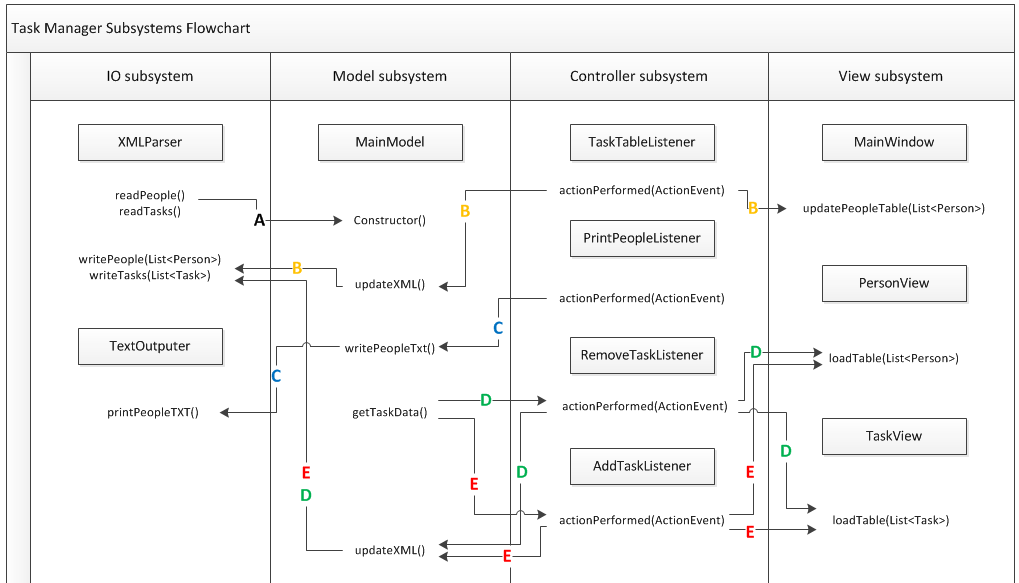
\includegraphics[scale=.6]{Diagrams/subsystem_flowchart.png} \end{center}
\caption{Subsystem Interface Flowchart}
\label{fig:sub-flow-diagram2}
\end{figure}

\begin{figure}[htbp]
\begin{center} 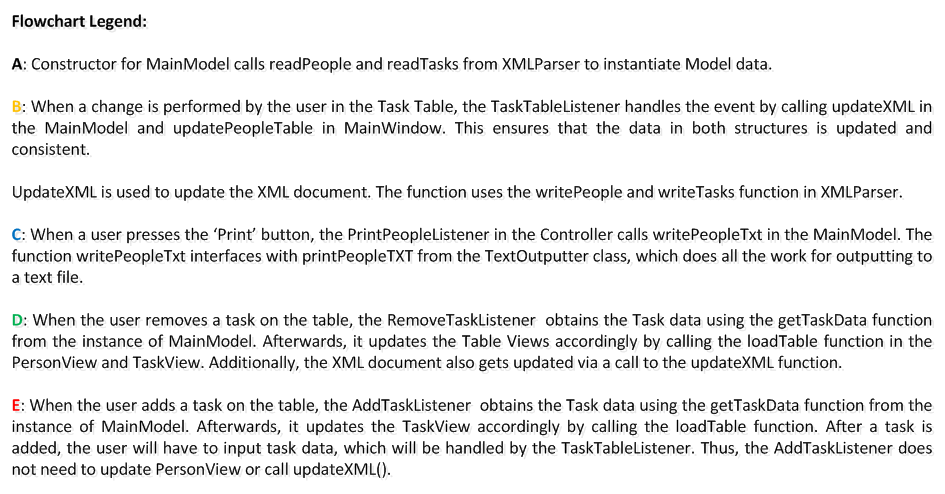
\includegraphics[scale=.65]{Diagrams/legend.png} \end{center}
\caption{Flowchart Legend}
\label{fig:legend}
\end{figure}

\section{Detailed Design} \label{sec:detail}

As stated previously, the system is composed of the Model, View and Controller subsystems.

\subsection{Model Subsystem}

\subsubsection{Detailed Design Diagram}

Please refer to Figure 4.
\begin{figure}[htbp]
\begin{center} 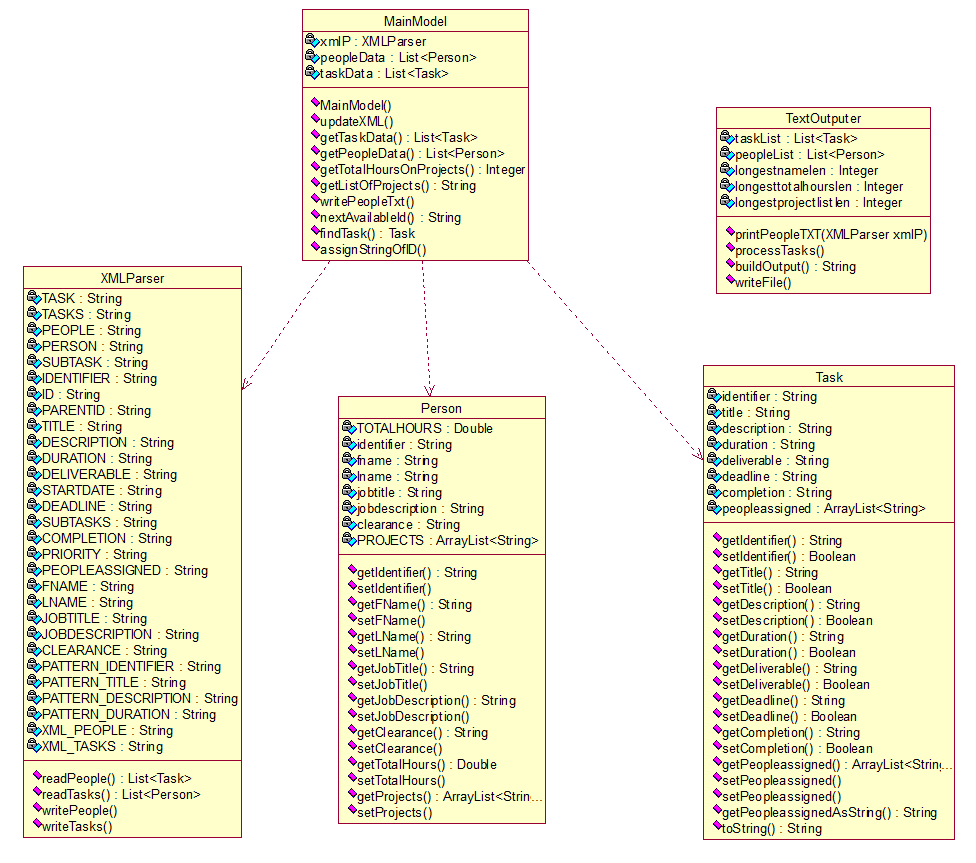
\includegraphics[scale=.7]{Diagrams/model_diagram.png} \end{center}
\caption{Model Design Diagram}
\label{fig:model-diagram1}
\end{figure}

\subsubsection{Units Description}

{\bf MainModel}
\begin{quote}
{\bf Description}\\
This class contains the XMLParser class (part of our I/O Subsystem), TextOutputer class (also part of I/O subsysem, responsible for wrtiting to an XML file). It also contains Person and Task classes. The purpose of this class is to group Person and Tasks data into same class and add functionality for writing that data to a file (I/O subsystem).\\\\
{\bf Attributes:}\\
\texttt{XMLParser xmlP}: \emph{The XML Parser}\\
\texttt{List<Person> peopleData}: \emph{List of persons in the XML file}\\
\texttt{List<Task> taskData}: \emph{List of tasks in the XML file}\\\\
{\bf Methods:}\\
\texttt{MainModel()}: \emph{Constructor}\\
\texttt{void updateXML()}: \emph{writes to XML file using XMLParser's \texttt{writePeople} and \texttt{writeTasks} methods}\\
\texttt{void writePeopleTxt()}: \emph{calls TextOutputer's \texttt{printPeopleTXT(xmlP)} method}\\
\texttt{Task findTask(String)}: \emph{Find a task by id from the \texttt{taskData} List}\\
\texttt{List<Task> getTaskData()}: \emph{getter}\\
\texttt{List<Person> getPeopleData()}: \emph{getter}\\
\texttt{int getTotalHoursOnProjects(String)}: \emph{gets Person's total hours}\\
\texttt{void writePeopleTxt()}: \emph{writes xmlParser to file using TextOutputer's static function}\\
\texttt{String nextAvailableId()}: \emph{Gets the next available ID (from the list of Tasks) when creating a new Task}\\
\texttt{String getListOfProjects(String)}: \emph{Gets the list of Tasks in a string, separated by a comma `,'.}\\
\texttt{void assignStringOfID(Task task, String data)}: \emph{When assigning new people to a Task, it validates the format of string ids and assigns new People to a Task}
\end{quote}
 
{\bf XMLParser}
\begin{quote}
{\bf Description}\\
This class parses people.xml and tasks.xml files and extracts appropriate data. It also writes to XML files.\\\\
{\bf Attributes:(Tags used to extract information when parsing)}\\
\texttt{String TASK}\\
\texttt{String TASKS}\\
\texttt{String PEOPLE}\\
\texttt{String PERSON}\\
\texttt{String IDENTIFIER}\\
\texttt{String ID}\\
\texttt{String PARENTID}\\
\texttt{String TITLE}\\
\texttt{String DESCRIPTION}\\
\texttt{String DURATION}\\
\texttt{String DELIVERABLE}\\
\texttt{String STARTDATE}\\
\texttt{String DEADLINE}\\
\texttt{String SUBTASKS}\\
\texttt{String COMPLETION}\\
\texttt{String PRIORITY}\\
\texttt{String PEOPLEASSIGNED}\\
\texttt{String FNAME}\\
\texttt{String LNAME}\\
\texttt{String JOBTITLE}\\
\texttt{String JOBDESCRIPTION}\\
\texttt{String CLEARANCE}\\
\texttt{String PATTERN\_IDENTIFIER}\\
\texttt{String PATTERN\_TITLE}\\
\texttt{String PATTERN\_DESCRIPTION}\\
\texttt{String PATTERN\_DURATION}\\
\texttt{String XML\_PEOPLE}\\
\texttt{String XML\_TASKS}\\
\texttt{String IDENTIFIER}\\\\
{\bf Methods:}\\
\texttt{void writeTasks(List<Task>)}: \emph{receives list of tasks and writes them to XML file}\\
\texttt{void writePeople(List<Person>)}: \emph{receives list of people and writes them to XML file}\\
\texttt{List<Task> readTasks()}: \emph{parses XML file and reads in tasks information, returning List of tasks}\\
\texttt{List<Person> readPeople()}: \emph{parses XML file and reads in people information, reurning List of people}
\end{quote}
 
{\bf TextOutputer}
\begin{quote}
{\bf Description}\\
This class formats and writes data (People) to people.txt\\\\
{\bf Attributes:}\\
\texttt{List<Task> taskList}\\
\texttt{List<Person> peopleList}\\
\texttt{int longestnamelen}\\
\texttt{int longesttotalhourslen}\\
\texttt{int longestprojectlistlen }\\\\

\pagebreak

{\bf Methods:}\\
\texttt{void printPeopleTXT(XMLParser)}: \emph{Writes new data to file using \texttt{writeFile} by first reading it from XMLParser, building output then calling \texttt{writeFile}.}\\
\texttt{void processTasks() }\\
\texttt{String buildOutput()}: \emph{Builds output string from list of Tasks and Persons and returns the string} \\
\texttt{void writeFile(String output)}: \emph{Gets the string and writes it to people.txt}
\end{quote} 

{\bf Person}
\begin{quote}
{\bf Description}\\
This class abstracts and encapsulates People data.\\\\
{\bf Attributes: (Setters and getters)}\\
\texttt{double TOTALHOURS}\\
\texttt{ArrayList<String> PROJECTS}\\
\texttt{String identifier}\\
\texttt{String fname}\\
\texttt{String lname}\\
\texttt{String jobtitle}\\
\texttt{String jobdescription}\\
\texttt{String clearance}\\\\
{\bf Methods:}\\
\texttt{String getIdentifier() }\\
\texttt{void setIdentifier(String) }\\
\texttt{String getFName() }\\
\texttt{void setFName(String) }\\
\texttt{String getLName() }\\
\texttt{void setLName(String) }\\
\texttt{String getJobTitle() }\\
\texttt{void setJobTitle(String) }\\
\texttt{String getJobDescription() }\\
\texttt{void setJobDescription(String) }\\
\texttt{String  getClearance() }\\
\texttt{void setClearance(String) }\\
\texttt{double getTotalHours() }\\
\texttt{void setTotalHours(double)  }\\
\texttt{ArrayList<String> getProjects()  }\\
\texttt{void setProjects(String) }\\
\texttt{String toString()}: \emph{Overrides \texttt{toString()} method and returns a list of attributes and their values, separated by `,' comma}
\end{quote}

\pagebreak
 
{\bf Task}
\begin{quote}
{\bf Description}\\
This class abstracts and encapsulates Task data.\\\\
{\bf Attributes: (Setters and getters)}\\
\texttt{String identifier}\\
\texttt{String title}\\
\texttt{String description}\\
\texttt{String duration}\\
\texttt{String deliverable}\\
\texttt{String deadline}\\
\texttt{String completion}\\
\texttt{ArrayList<String> peopleassigned }\\\\
{\bf Methods:}\\
\texttt{public Task()}:   \emph{Default Constructor}\\
\texttt{public Task(String)}:   \emph{Constructor}\\
\texttt{String getIdentifier()  }\\
\texttt{boolean setIdentifier(String)  }\\
\texttt{String getTitle()  }\\
\texttt{boolean setTitle(String)  }\\
\texttt{String getDescription()  }\\
\texttt{boolean setDescription(String)  }\\
\texttt{String getDuration() }\\
\texttt{boolean setDuration(String)  }\\
\texttt{String getDeliverable() }\\
\texttt{boolean setDeliverable(String) }\\
\texttt{String getDeadline()  }\\
\texttt{boolean setDeadline(String) }\\
\texttt{String getCompletion() }\\
\texttt{boolean setCompletion(String) }\\
\texttt{ArrayList<String> getPeopleassigned() }\\
\texttt{void setPeopleassigned(String)  }\\
\texttt{void setPeopleassigned(ArrayList<String>) }\\
\texttt{String getPeopleassignedAsString()  }\\
\texttt{String toString()}: \emph{Overrides \texttt{toString()} method and returns a list of attributes and their values, separated by `,' comma}
\end{quote}

\subsection{View Subsystem}

\subsubsection{Detailed Design Diagram}

Please refer to Figure 5.\\\\\\\\\\

\begin{figure}[htbp]
\begin{center} 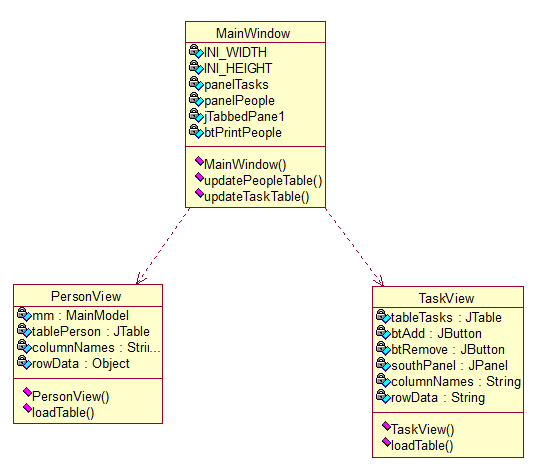
\includegraphics[scale=.55]{Diagrams/view_diagram.png} \end{center}
\caption{View Design Diagram}
\label{fig:model-diagram2}
\end{figure}

\subsubsection{Units Description}

{\bf TaskView}
\begin{quote}
{\bf Description}\\
This class is responsible for displaying the list of tasks in a table format. It is initially called by MainWindow and is passed an object, of type MainModel, from which it reads all the tasks using the \texttt{LoadTable()} method.\\\\
{\bf Attributes:}\\
\texttt{JButton btAdd}\\
\texttt{JButton btRemove}\\
\texttt{String[] columnNames}\\
\texttt{String[][] rowData}\\
\texttt{JPanel southPanel}\\
\texttt{JTable tableTasks}\\\\
{\bf Methods:}\\
\texttt{Taskview(List<Task> taskData)}:  \emph{Constructor}\\
\texttt{void loadTable(List<Task>)}: \emph{ Gets the list of tasks from the model and populates the table with data}
\end{quote}

{\bf PersonView}
\begin{quote}
{\bf Description}\\
This class is responsible for displaying the list of people in a table format. It is initially called by MainWindow and is passed a list of people from which it reads all the datausing the \texttt{loadTable()} method.\\\\
{\bf Attributes:}\\
\texttt{String[] columnNames}\\
\texttt{MainModel mm}\\
\texttt{Object[][] rowData}\\
\texttt{JTable tablePerson}\\\\
{\bf Methods:}\\
\texttt{Personview(MainModel mm)}:  \emph{Constructor}\\
\texttt{void loadTable(List<Person>)}:  \emph{Gets the list of people from the model and populates the table with the data}
\end{quote}

{\bf MainWindow}
\begin{quote}
{\bf Description}\\
This class creates the window that contains the Tasks and People tabs.  It sets the layout, buttons and panel at the bottom of the screen. In the event a button is pressed, this class does not handle the event.  A listener in the Controller catches the event and sends MainWindow the updated data.\\\\
{\bf Attributes:}\\
\texttt{int INI\_HEIGHT}\\
\texttt{int INI\_WIDTH}\\
\texttt{JButton btPrintPeople}\\
\texttt{JTabbedPane jTabbedPane1}\\
\texttt{PersonView panelPeople}\\
\texttt{TaskView panelTasks}\\\\
{\bf Methods:}\\
\texttt{MainWindow(MainModel mm)}:  \emph{Constructor}\\
\texttt{updatePeopleTable(List<Person>)}:  \emph{Calls Person's view \texttt{loadTable()} method, which gets the data from the model and loads into the table}\\
\texttt{updateTaskTable(List<Task>)}: \emph{Calls task's view \texttt{loadTable()} method, which gets the data from the model and loads it into the table}
\end{quote}

\subsection{Controller Subsystem}

\subsubsection{Detailed Design Diagram}

Please refer to Figure 6.

\begin{figure}[htbp]
\begin{center} 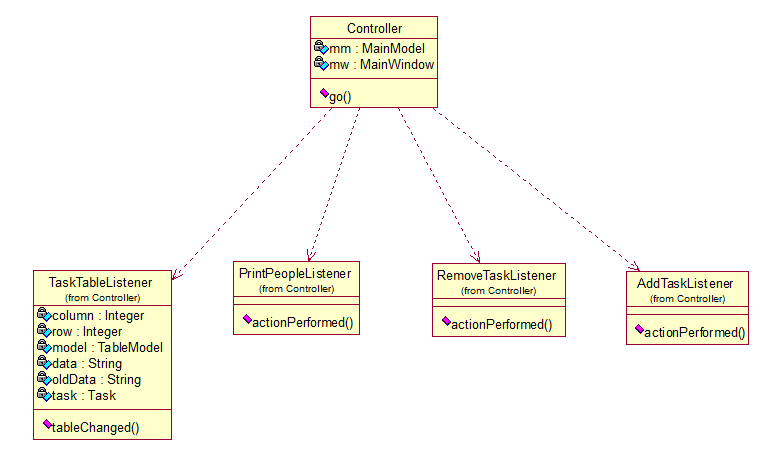
\includegraphics[scale=.55]{Diagrams/controller_diagram.png} \end{center}
\caption{Controller Design Diagram}
\label{fig:model-diagram3}
\end{figure}

\subsubsection{Units Description}

{\bf Controller}
\begin{quote}
{\bf Description}\\
This class contains MainModel varaible, MainWindow variable and 4 listeners. MainModel is a model attribute which has underlying data and methods to manipulate the data (read, update, write to files). The MainWindow is the main application window class, which contains 2 views: PersonView and TaskView.\\\\
{\bf Attributes:}\\
\texttt{MainModel mm}\\
\texttt{Mainwindow mw}\\ 
\texttt{class TaskTableListener}: \emph{The object of this class is attached to TableModelListener of the \texttt{jTable}.  When the table is edited the listener\\ \texttt{tableChanged(TableModelEvent e)} catches the event, which first updates the model, writes new changes to XML by calling \texttt{mm.updateXML()} in the MainModel and then reloads the table with new data by calling\\ \texttt{mw.updatePeopleTable(mm.getPeopleData())} in the MainWindow.  }\\
\texttt{class PrintPeopleListener}: \emph{The object of this class is attached to Action Listener of the \texttt{btPrintPeople} button in the MainWindow \texttt{mw}. When user presses on the button ``Print People Table", the event is caught and this class calls the method \texttt{mm.writePeopleTxt()} in the MainModel.}\\
\texttt{class RemoveTaskListener} \emph{The object of this class is attached to the action listener of the \texttt{btRemove} button in the MainWindow \texttt{mw}.  When users presses on the button ``Remove Task", this event is caught and this class calls finds the Task which is about to be removed in the model,  removes it, then updates both Tables, and also writes new changes to XML file by calling \texttt{mm.updateXML()}.}\\
\texttt{class AddTaskListener}\emph{The object of this class is attached to the action listener of the \texttt{btAdd} button in the MainWindow \texttt{mw}. When user presses on the button ``Add Task", this event is caught and this class creates a new Task, adds it to the model, updates both People and Tasks tables, and also writes new data to XML file by calling \texttt{mm.updateXML()}.}\\\\
{\bf Methods:}\\
\texttt{void updatePeopleTable(List<Person> pList)}: \emph{Creates and initializes a new \texttt{MainModel} and creates and initializes a new MainWindow which contains two panels: PersonView and TaskView.}
\end{quote}

\section{Dynamic Design Scenarios}

The following sequence diagrams represent three execution scenarios of the system. Each diagram follows the flow of data through the system design to achieve a system-level service. Note that the execution scenario for removing a task is almost identical to the scenario for adding a task.

\begin{figure}[htbp]
\begin{center} 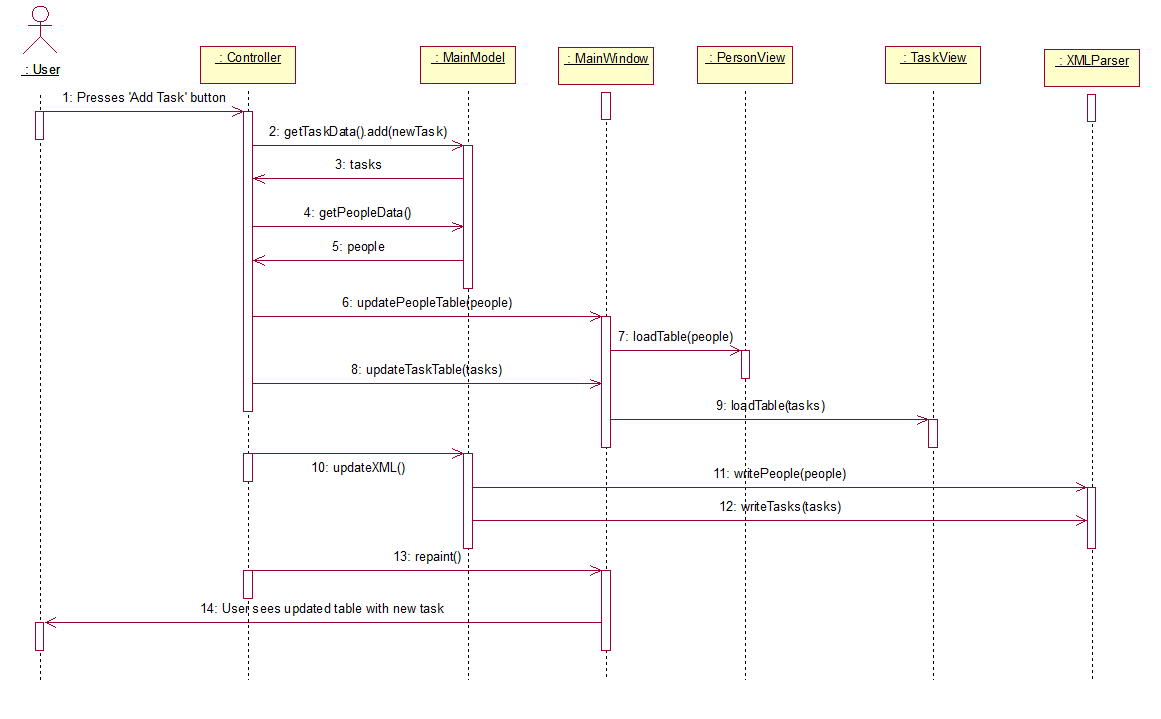
\includegraphics[scale=.55]{Diagrams/add_task_diagram.png} \end{center}
\caption{Execution Scenario: User adds task to table}
\label{fig:add-task-diagram}
\end{figure}

\begin{figure}[htbp]
\begin{center} 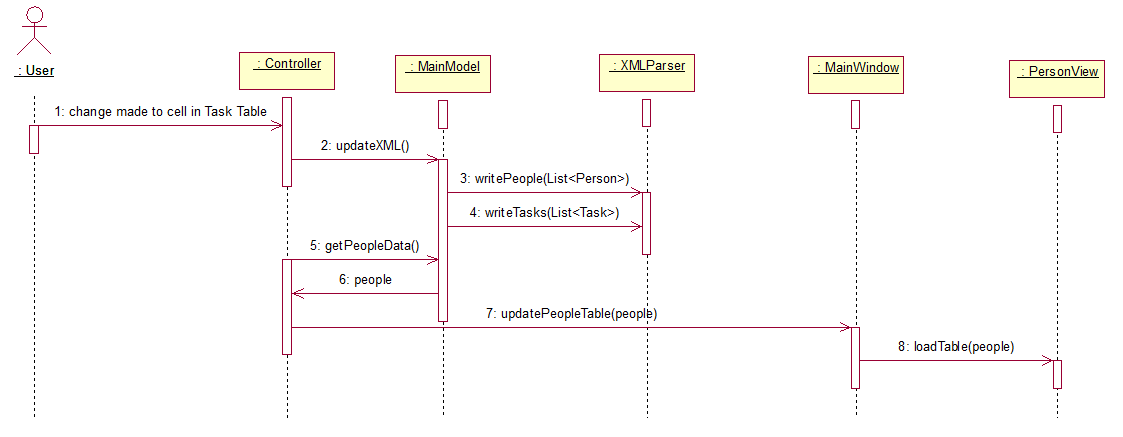
\includegraphics[scale=.55]{Diagrams/change_cell_diagram.png} \end{center}
\caption{Execution Scenario: User changes cell on table}
\label{fig:change-cell-diagram}
\end{figure}

\begin{figure}[htbp]
\begin{center} 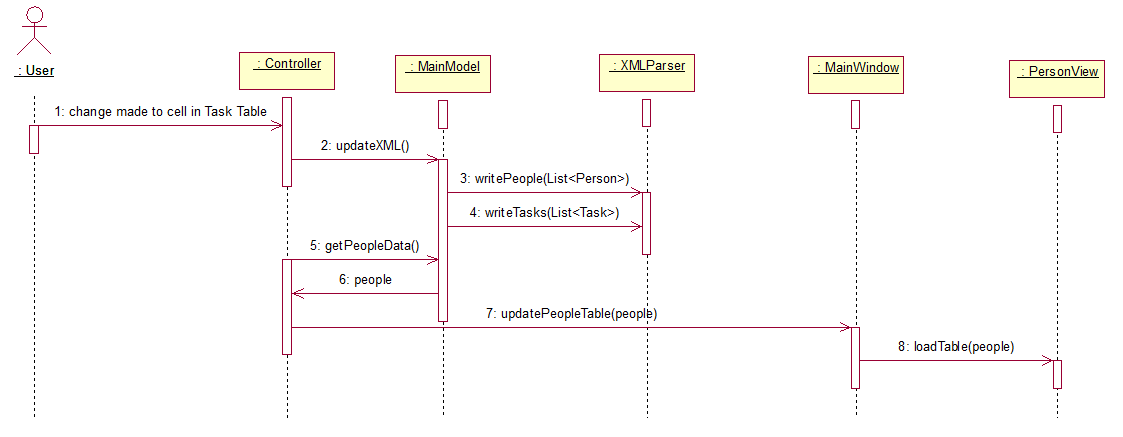
\includegraphics[scale=.55]{Diagrams/change_cell_diagram.png} \end{center}
\caption{Execution Scenario: User requests to print text file}
\label{fig:print-text-diagram}
\end{figure}

\end{document}
